%% Style 16: Infographic Style - Skill bars, timeline for experience, visual elements
\documentclass[10pt,a4paper]{article}
\usepackage[utf8]{inputenc}
\usepackage[T1]{fontenc}
\usepackage[left=0.5in,right=0.5in,top=0.4in,bottom=0.4in]{geometry}
\usepackage[usenames,dvipsnames]{xcolor}
\usepackage{tikz}
\usepackage{fontawesome5}
\usepackage{enumitem}
\usepackage{titlesec}
\usepackage[hidelinks]{hyperref}
\usepackage{lmodern}

\usetikzlibrary{calc}

\definecolor{primary}{HTML}{2C3E50}
\definecolor{accent}{HTML}{E74C3C}
\definecolor{timeline}{HTML}{3498DB}
\definecolor{skillbg}{HTML}{ECF0F1}
\definecolor{skillfill}{HTML}{3498DB}
\definecolor{text}{HTML}{2C3E50}

\pagestyle{empty}
\color{text}

\titleformat{\section}{\color{primary}\large\bfseries\scshape}{}{0em}{}
\titlespacing{\section}{0pt}{10pt}{4pt}

% Skill bar
\newcommand{\infoskillbar}[2]{%
  \noindent\small #1 \hfill \small #2\%\par\vspace{2pt}%
  \begin{tikzpicture}
    \fill[skillbg, rounded corners=2pt] (0,0) rectangle (5.0cm,0.2cm);
    \fill[skillfill, rounded corners=2pt] (0,0) rectangle ({5.0*#2/100},0.2cm);
  \end{tikzpicture}\par\vspace{4pt}%
}

% Timeline entry
\newcommand{\timelineentry}[5]{%
  \noindent\begin{tikzpicture}
    \fill[timeline] (0,0) circle (4pt);
    \draw[timeline, line width=1pt] (0,-4pt) -- (0,-0.8cm);
    \node[right, anchor=west, text width=14cm] at (0.4cm,0) {%
      \textbf{\color{primary}#1} -- \textit{#2}\\
      {\small\color{timeline}#3 | #4}\\[2pt]
      {\small #5}%
    };
  \end{tikzpicture}\par\vspace{4pt}%
}

\begin{document}

% Header
\begin{center}

\begin{tikzpicture}
\fill[primary, rounded corners=4pt] (0,0) rectangle (\textwidth,2.0cm);
\node[anchor=center, text=white] at ({\textwidth/2},1.3cm) {\fontsize{24pt}{28pt}\selectfont\textbf{Arjun Mehta}};
\node[anchor=center, text=white] at ({\textwidth/2},0.5cm) {\large Senior Software Engineer | Bangalore, India};
\end{tikzpicture}
\end{center}
\vspace{4pt}

% Contact bar
\begin{center}
\small\color{primary}
\faEnvelope\ arjun.mehta@email.com \quad
\faPhone\ +91-98765-43210 \quad
\faLinkedin\ arjunmehta \quad
\faGithub\ arjunmehta
\end{center}
\vspace{6pt}

% Two column layout
\noindent\begin{minipage}[t]{0.62\textwidth}

\section{\faHistory\ Experience Timeline}
\vspace{4pt}

\timelineentry{Senior Software Engineer}{AWS}{Jan 2023 -- Present}{Bangalore}{%
Designed distributed microservices (50K+ req/sec). Led monolith migration reducing latency 40\%. Mentored 4 engineers.}

\timelineentry{Software Engineer}{Microsoft}{Jun 2020 -- Dec 2022}{Hyderabad}{%
Built 10TB+ daily data pipeline. REST APIs for 1M+ users at 99.9\% uptime. Cut CI/CD time by 60\%.}

\vspace{6pt}
\section{\faRocket\ Projects}
\vspace{4pt}

\timelineentry{Distributed Task Scheduler}{Go, gRPC, Redis}{2023}{}{%
100K+ concurrent jobs. Raft consensus for leader election.}

\timelineentry{Analytics Dashboard}{React, D3.js, WebSocket}{2022}{}{%
Real-time streaming visualization, sub-second refresh.}

\vspace{6pt}
\section{\faGraduationCap\ Education}
\vspace{4pt}
\noindent
\begin{tikzpicture}
\fill[timeline] (0,0) circle (4pt);
\node[right, anchor=west] at (0.4cm,0) {\textbf{B.Tech Computer Science} -- IIT Bombay};
\node[right, anchor=west] at (0.4cm,-0.5cm) {\small 2016--2020 | GPA: 3.8/4.0};
\end{tikzpicture}

\end{minipage}%
\hfill%
\begin{minipage}[t]{0.34\textwidth}

\section{\faCogs\ Technical Skills}
\vspace{6pt}

\infoskillbar{Java}{92}
\infoskillbar{Python}{87}
\infoskillbar{Go}{82}
\infoskillbar{TypeScript}{78}
\infoskillbar{AWS}{90}
\infoskillbar{Kubernetes}{85}
\infoskillbar{System Design}{88}
\infoskillbar{Kafka/Spark}{83}
\infoskillbar{React}{76}
\infoskillbar{Docker}{88}
\infoskillbar{Terraform}{75}

\vspace{8pt}
\section{\faTrophy\ Highlights}
\vspace{4pt}
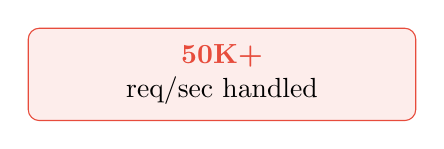
\begin{tikzpicture}
\node[draw=accent, rounded corners=4pt, fill=accent!10, text width=4.5cm, inner sep=6pt, align=center] {
  \textbf{\color{accent}50K+}\\req/sec handled
};
\end{tikzpicture}
\vspace{4pt}
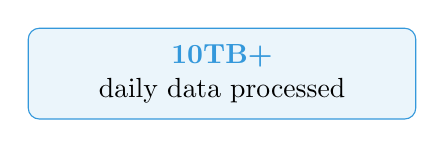
\begin{tikzpicture}
\node[draw=timeline, rounded corners=4pt, fill=timeline!10, text width=4.5cm, inner sep=6pt, align=center] {
  \textbf{\color{timeline}10TB+}\\daily data processed
};
\end{tikzpicture}
\vspace{4pt}

\begin{tikzpicture}
\node[draw=primary, rounded corners=4pt, fill=primary!10, text width=4.5cm, inner sep=6pt, align=center] {
  \textbf{\color{primary}99.9\%}\\uptime SLA
};
\end{tikzpicture}

\end{minipage}

\end{document}
